\documentclass[aspectratio=43,scheme=plain]{ctexbeamer}
%\usepackage{xeCJK}
\setCJKmainfont{IPAexGothic}

%\usetheme{Antibes}
%\setbeamertemplate{navigation symbols}{\thepage}
%\setbeamertemplate{caption}[numbered]

\usetheme{trigon}
\trigonset{titlestyle=style2,
	sectionpage=none,
	headingcolor=theme,
	numbering=fraction,
	block=fill
}

%\usetheme[showmaxslides,customfont,nofooter]{pureminimalistic}
%\renewcommand{\logotitle}{}
%\renewcommand{\logoheader}{}
%\renewcommand{\logofooter}{}

%\usetheme[numbering=fraction,progressbar=frametitle,sectionpage=none,block=fill,subsectionpage=none]{metropolis}
\usepackage{pgfpages}
%\pgfpagesuselayout{4 on 1}[a4paper,landscape]
%\setbeameroption{show notes on second screen=right}

\AtBeginSection[]{
	\begin{frame}{Contents}
%		\thispagestyle{empty}
		\tableofcontents[currentsection]
\end{frame}}
\usefonttheme{professionalfonts}

\usepackage{siunitx}
\usepackage[version=4]{mhchem}
\usepackage{amsmath}
\usepackage{amssymb}
\usepackage{amsfonts}
\usepackage{metalogo}
\usepackage{appendix}
\usepackage{xcolor}
%\pagecolor[RGB]{46,46,46}
%\color[RGB]{248,248,248}
\usepackage{framed}
\usepackage{tabularx}
\usepackage{colortbl}
\usepackage{enumerate}
\usepackage{wrapfig2}
\usepackage{graphicx}
\usepackage{subfigure} 
\usepackage{float} 
\usepackage{tikz}
\usepackage{qrcode}

\renewcommand{\appendixtocname}{付録}
\renewcommand{\appendixpagename}{付録}
\renewcommand{\contentsname}{目次}
\renewcommand{\figurename}{Fig.}

\usepackage[hyperref=true,backend=biber,url=true,doi=true,dateabbrev=true,backref=true,style=numeric-comp,maxnames=15]{biblatex}
\DeclareFieldFormat{biblabeldate}{\mkbibparens{\mkbibbold{#1}}}
\DeclareFieldFormat[article,periodical]{volume}{\mkbibbold{#1}}
\renewbibmacro{in:}{}
\addbibresource{reference.bib}%导入bib文件。

%\usepackage{hyperref}
\hypersetup{
	bookmarksnumbered=true,
	colorlinks=false,
	linkcolor=black,
	urlcolor=black,
	citecolor=black,
	pdfauthor={B4},
	pdfcreator={XYX},
	pdftitle={Machine time report},
	pdfsubject={Galvano, },
	pdfkeywords={Exercise experiments}
}


\title{練習実験報告}
\author{肖宇笑}
\date{\today}
\begin{document}
%	\maketitle 						   %for Metropolis
	\titleframe						    %for Trigon
%	\begin{frame}                      %for Antibes
%	\thispagestyle{empty}         %for Antibes
%	\titlepage                             %for Antibes
%	\end{frame}                          %for Antibes
	\section{Glavano Sepctrum}	
	\begin{frame}{\insertsection}
		\begin{figure}[H]
			\centering
			\begin{tikzpicture}
					\onslide<1>{\node at (0,0){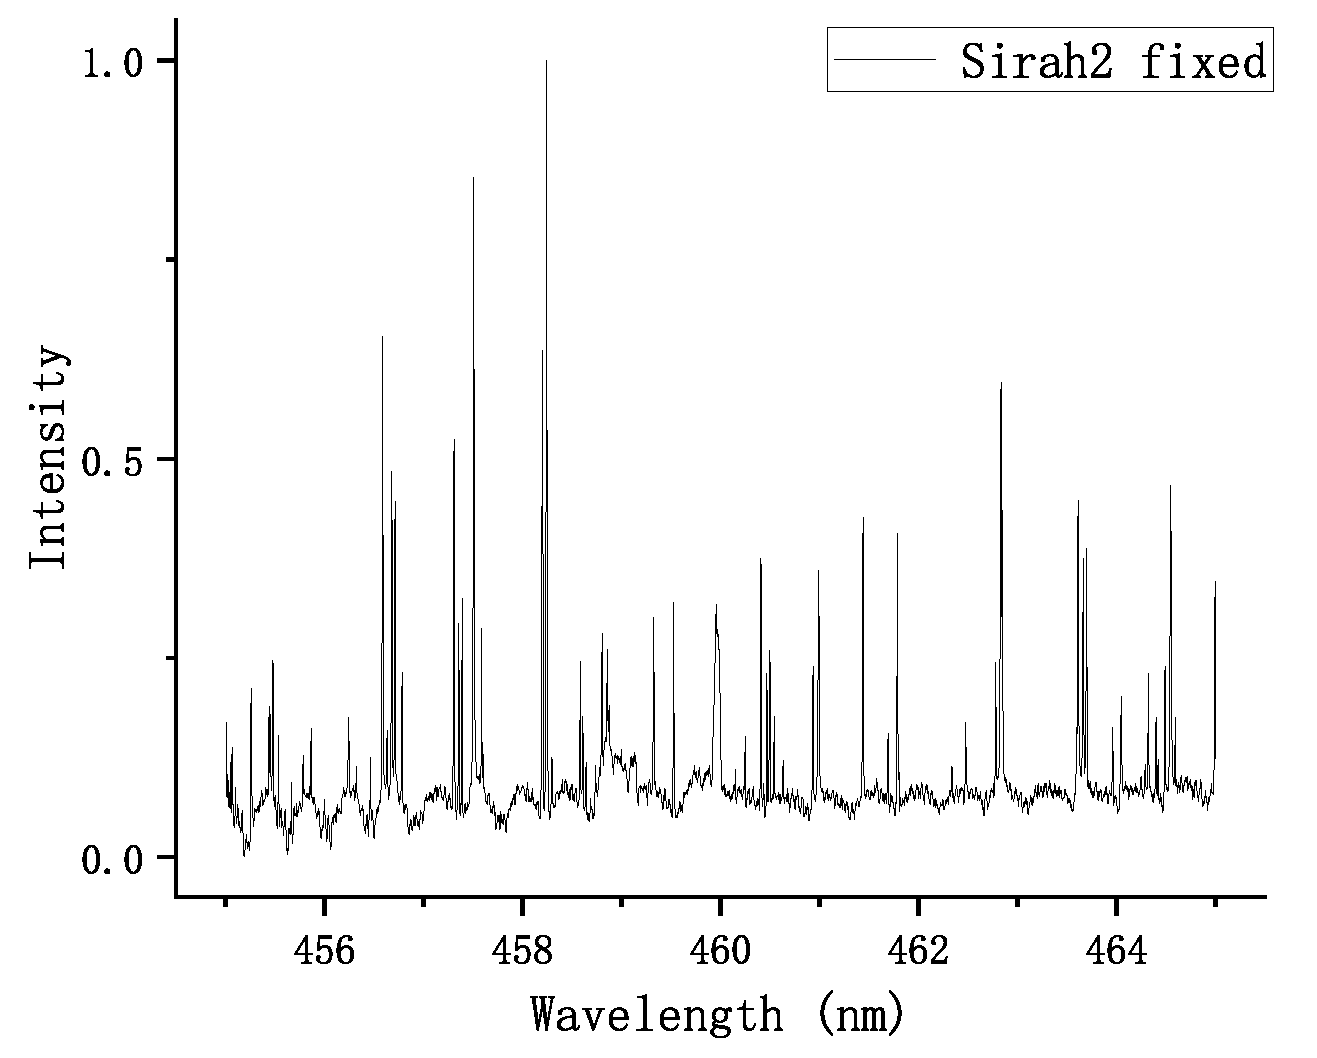
\includegraphics[width=0.6\textwidth]{sirah2fixed.eps}};}
					\onslide<2>{\node at (0,0){\includegraphics[width=0.6\textwidth]{wavelen_corrected.pdf}};}
			\end{tikzpicture}
			\caption{Wavelen. correction}
		\end{figure}
	\end{frame}
	\begin{frame}{\insertsection}{Correction}
		\begin{figure}[H]
			\centering
			\includegraphics[width=0.6\textwidth]{fitfunc.pdf}
			\caption{Correction function}
		\end{figure}
	\end{frame}
\section{REMPI scan}
\subsection{Selected peaks}
\begin{frame}{\insertsubsection}
\begin{figure}[H]
\centering
\begin{tikzpicture}
%	\draw (4,3.1) rectangle (4.03,3.295);
\draw (4,3.1) rectangle (4.1,3.2);
			\node at (0,0){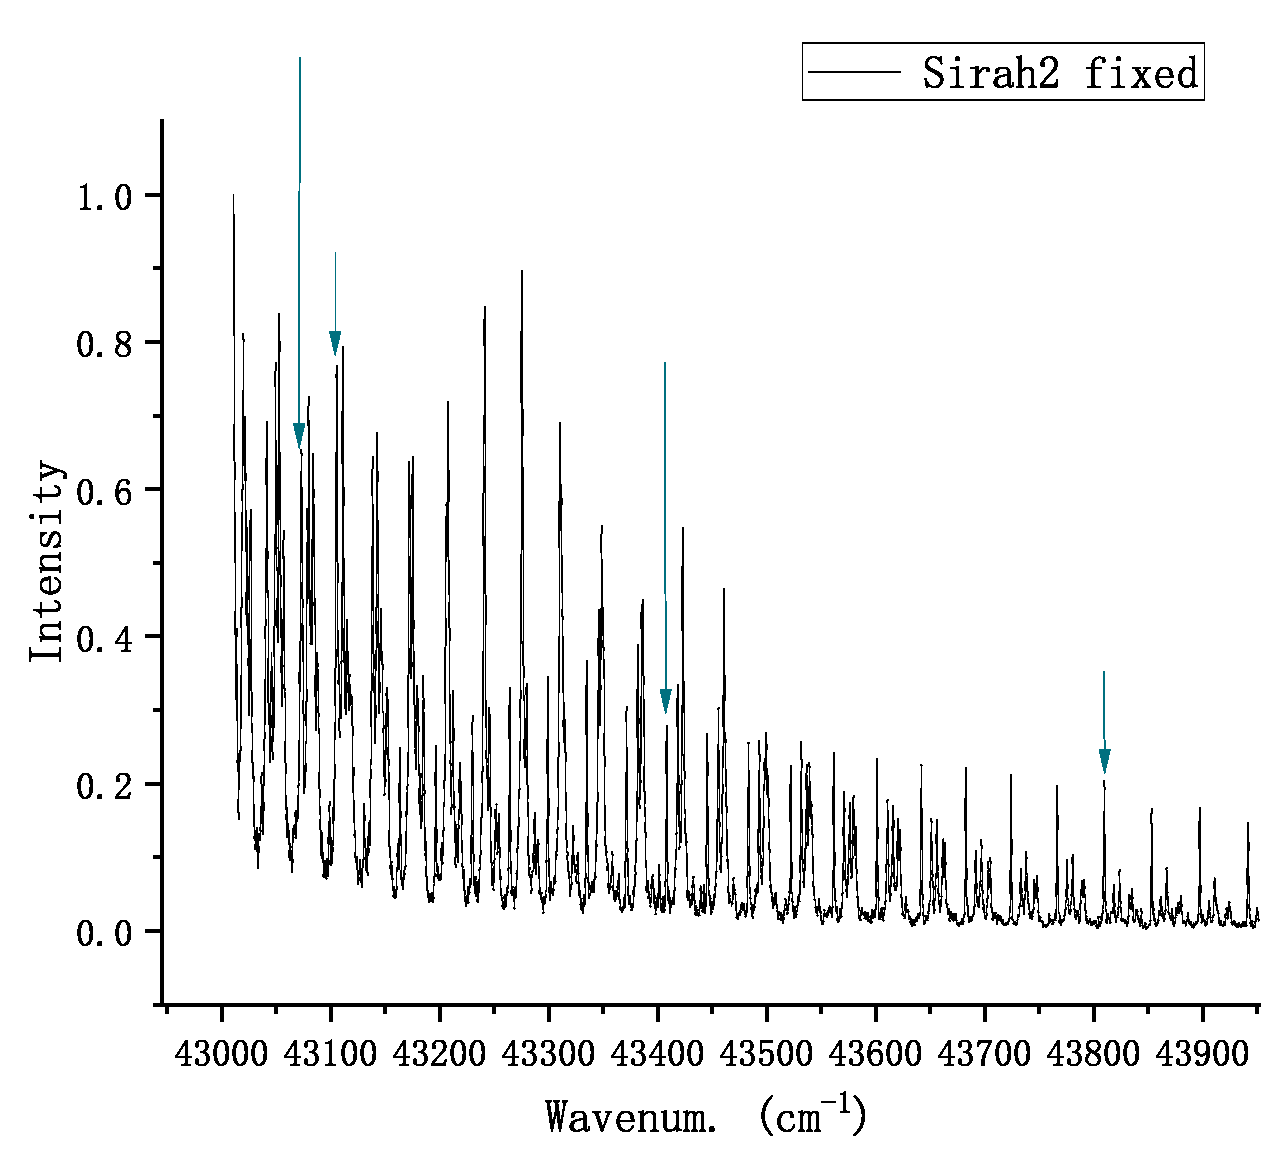
\includegraphics[width=0.6\textwidth]{scanmark.eps}};
			\filldraw[white] (-1.92,2.5) rectangle (-1.88,2.89);
			\node at (-1.5,2.7){\textcolor[RGB]{0,112,127}{$\num{464.455}\unit{\nano \meter}$}};
			\node at (-0.95,2){\textcolor[RGB]{0,112,127}{$\num{464.108}\unit{\nano \meter}$}};
			\node at (0.5,1.45){\textcolor[RGB]{0,112,127}{$\num{460.876}\unit{\nano \meter}$}};
			\node at (2.3,-0.25){\textcolor[RGB]{0,112,127}{$\num{456.653}\unit{\nano \meter}$}};
\end{tikzpicture}
\end{figure}
\end{frame}
\begin{frame}{Peak 1}
	\begin{figure}[H]
		\centering
		\begin{tikzpicture}
	\onslide<1>{\node at (0,0){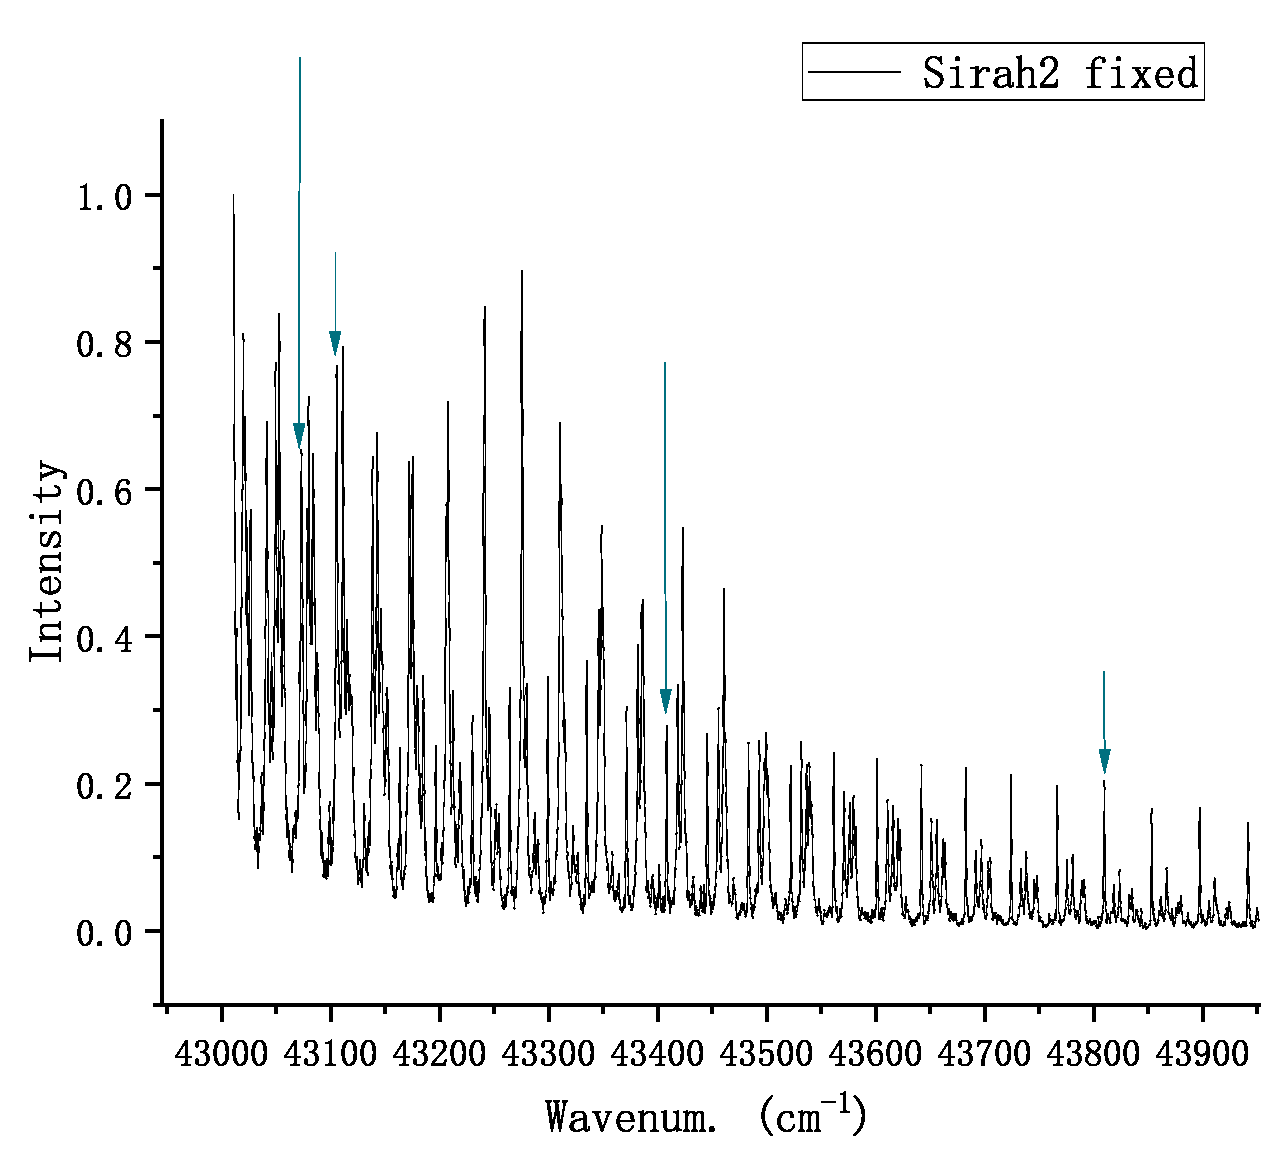
\includegraphics[width=0.6\textwidth]{scanmark.eps}};
	\filldraw[white] (-1.92,2.5) rectangle (-1.88,2.89);
	\node at (-1.5,2.7){\textcolor[RGB]{0,112,127}{$\num{464.455}\unit{\nano \meter}$}};
}
	\onslide<2>{\node at (-1.55,2){\includegraphics[width = 4cm]{gring_464355.eps}};
	\node at (2.45,2){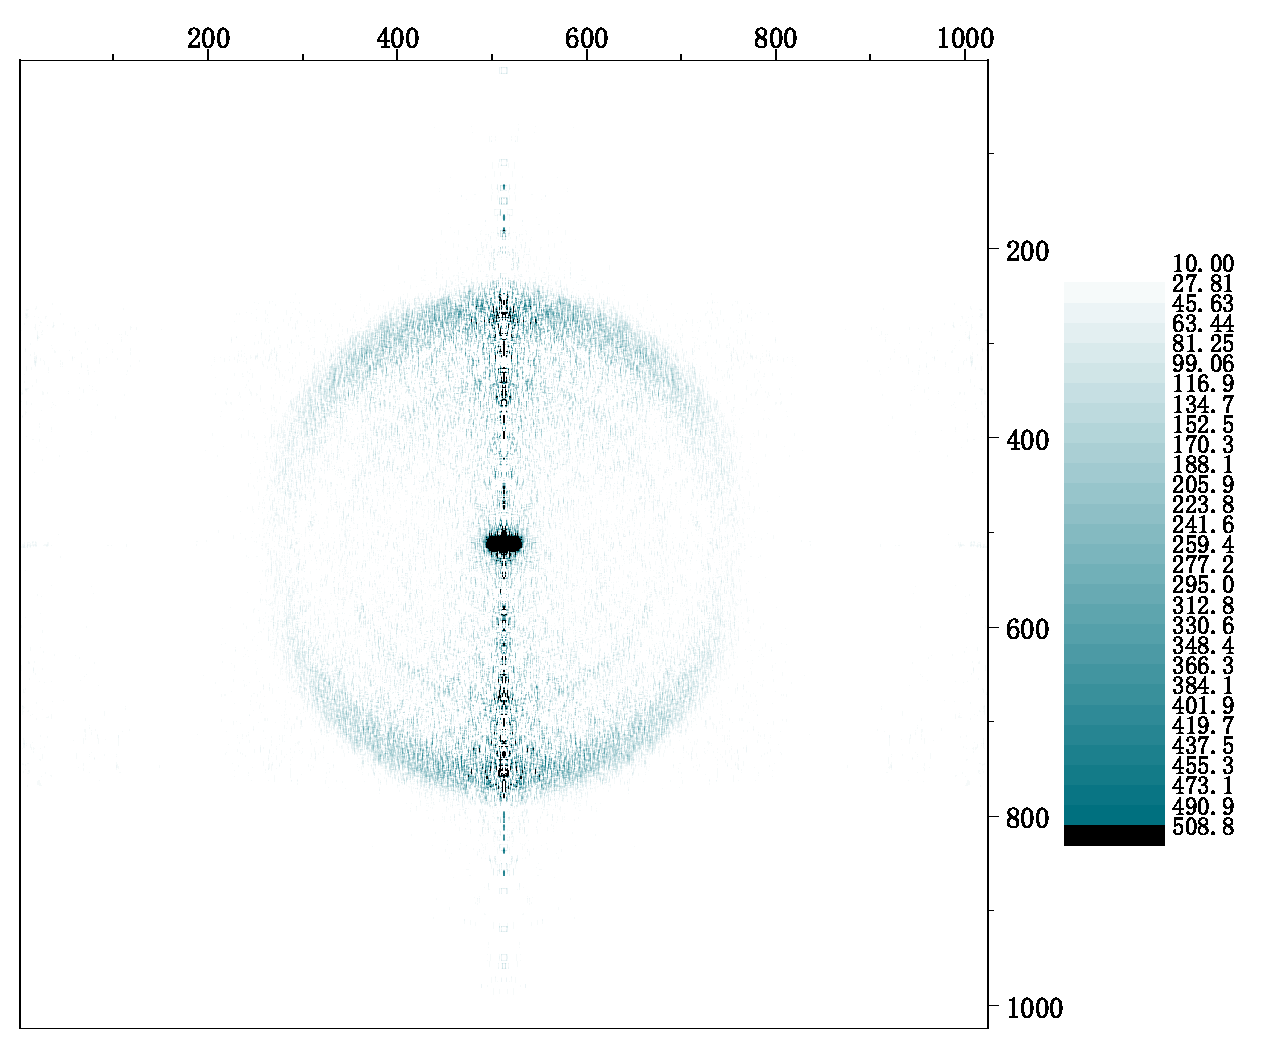
\includegraphics[width=4cm]{aring_464355.eps}};
	\node at (-2,-2){\includegraphics[width=4cm]{rdis_peak_464355.eps}};
	\node at (2,-2){\includegraphics[width=4cm]{adis_464355b.eps}};
	\node at (1.3,-3.2){\textcolor[RGB]{0,112,127}{\small $\beta \approx 1.52$}};
		\node at (-3.0,3.3){\textcolor[RGB]{0,112,127}{smear}};
	\node at (3.07,3.3){\textcolor[RGB]{0,112,127}{Abel${}^{-1}$}};}
\end{tikzpicture}
\end{figure}
\end{frame}
\begin{frame}{Peak 2}
	\begin{figure}[H]
		\centering
		\begin{tikzpicture}
	\onslide<1>{\node at (0,0){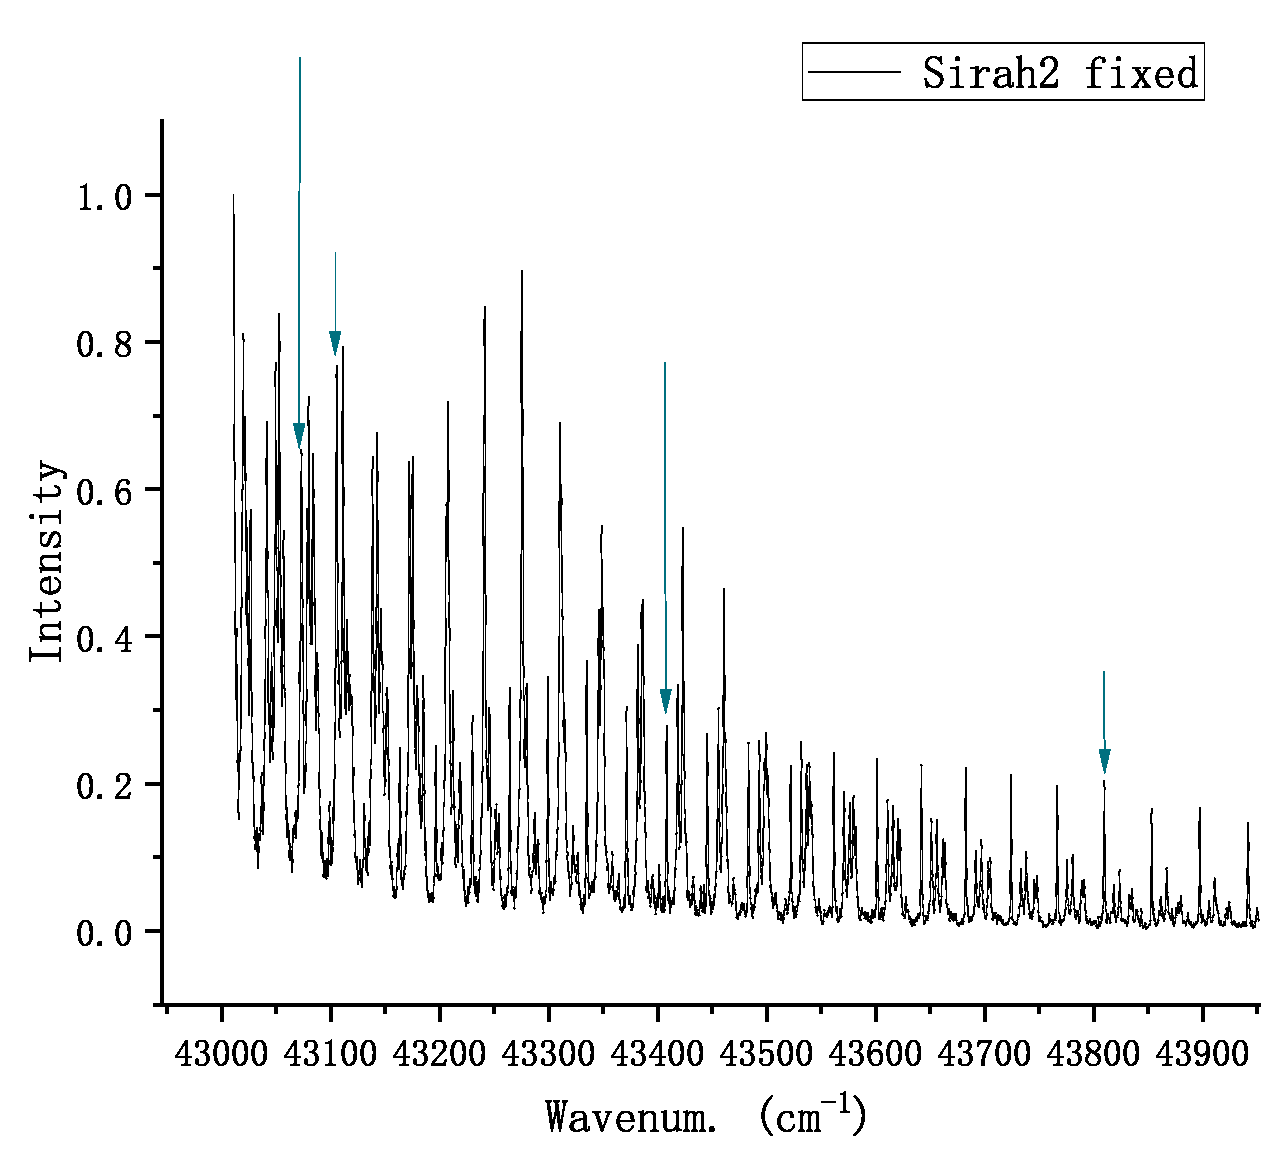
\includegraphics[width=0.6\textwidth]{scanmark.eps}};
	\filldraw[white] (-1.92,2.5) rectangle (-1.88,2.89);
			\node at (-0.95,2){\textcolor[RGB]{0,112,127}{$\num{464.108}\unit{\nano \meter}$}};
}
		\onslide<2>{\node at (-1.55,2){\includegraphics[width = 4cm]{gring_463985.eps}};
			\node at (2.45,2){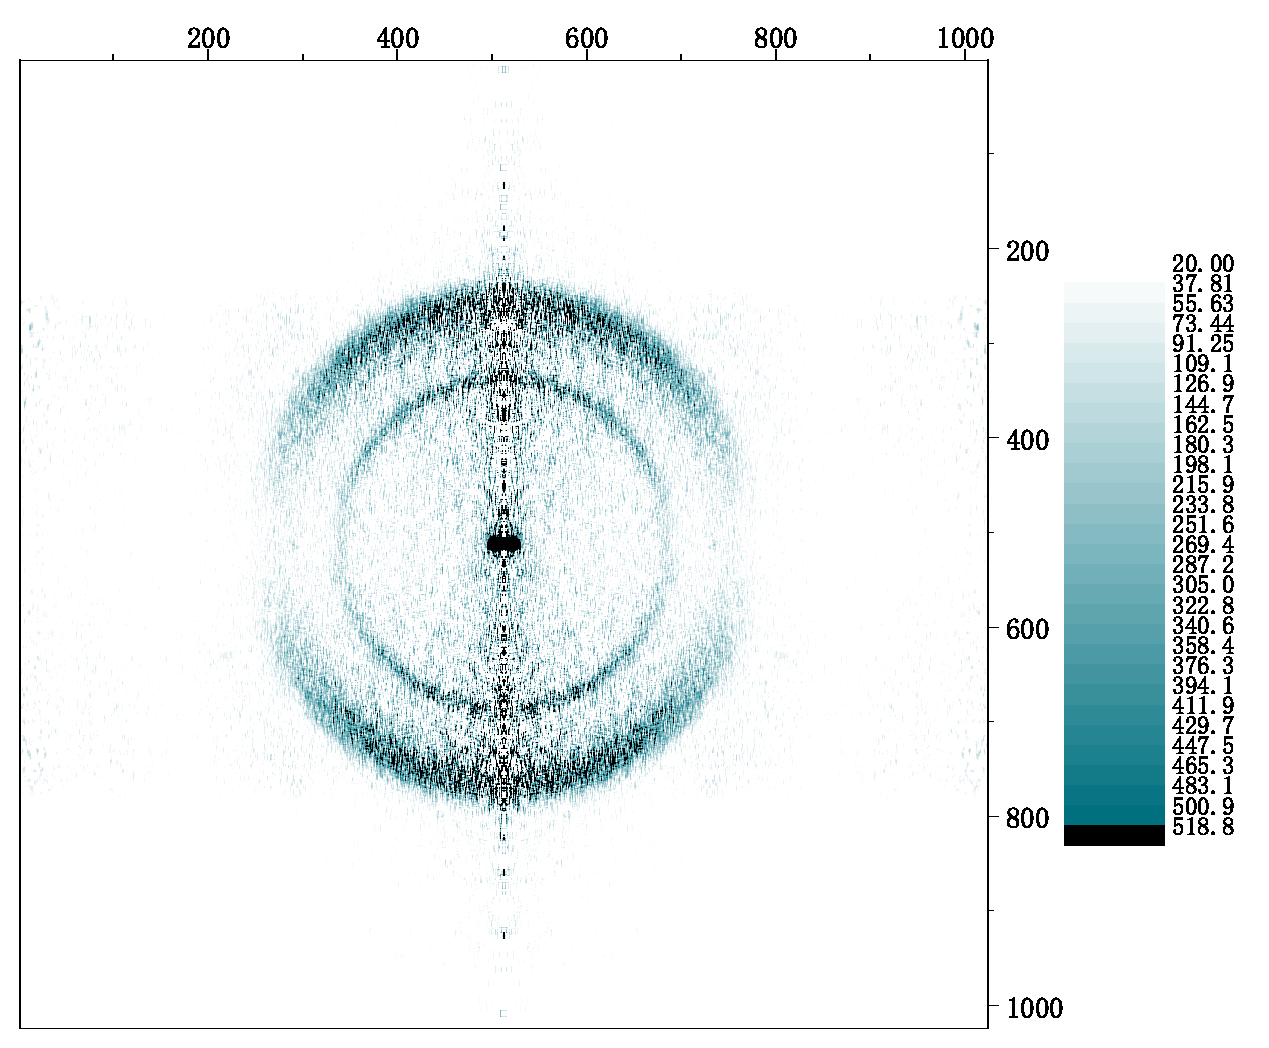
\includegraphics[width=4cm]{aring_463985.eps}};
			\node at (-2,-2){\includegraphics[width=4cm]{rdis_peak_463985.eps}};
			\node at (2,-2){\includegraphics[width=4cm]{adis_463985b.eps}};
			\node at (1.3,-3.2){\textcolor[RGB]{0,112,127}{\small $\beta \approx 1.23$}};
				\node at (-3.0,3.3){\textcolor[RGB]{0,112,127}{smear}};
			\node at (3.07,3.3){\textcolor[RGB]{0,112,127}{Abel${}^{-1}$}};}
\end{tikzpicture}
\end{figure}
\end{frame}
\begin{frame}{Peak 3}
\begin{figure}[H]
\centering
\begin{tikzpicture}
			\onslide<1>{\node at (0,0){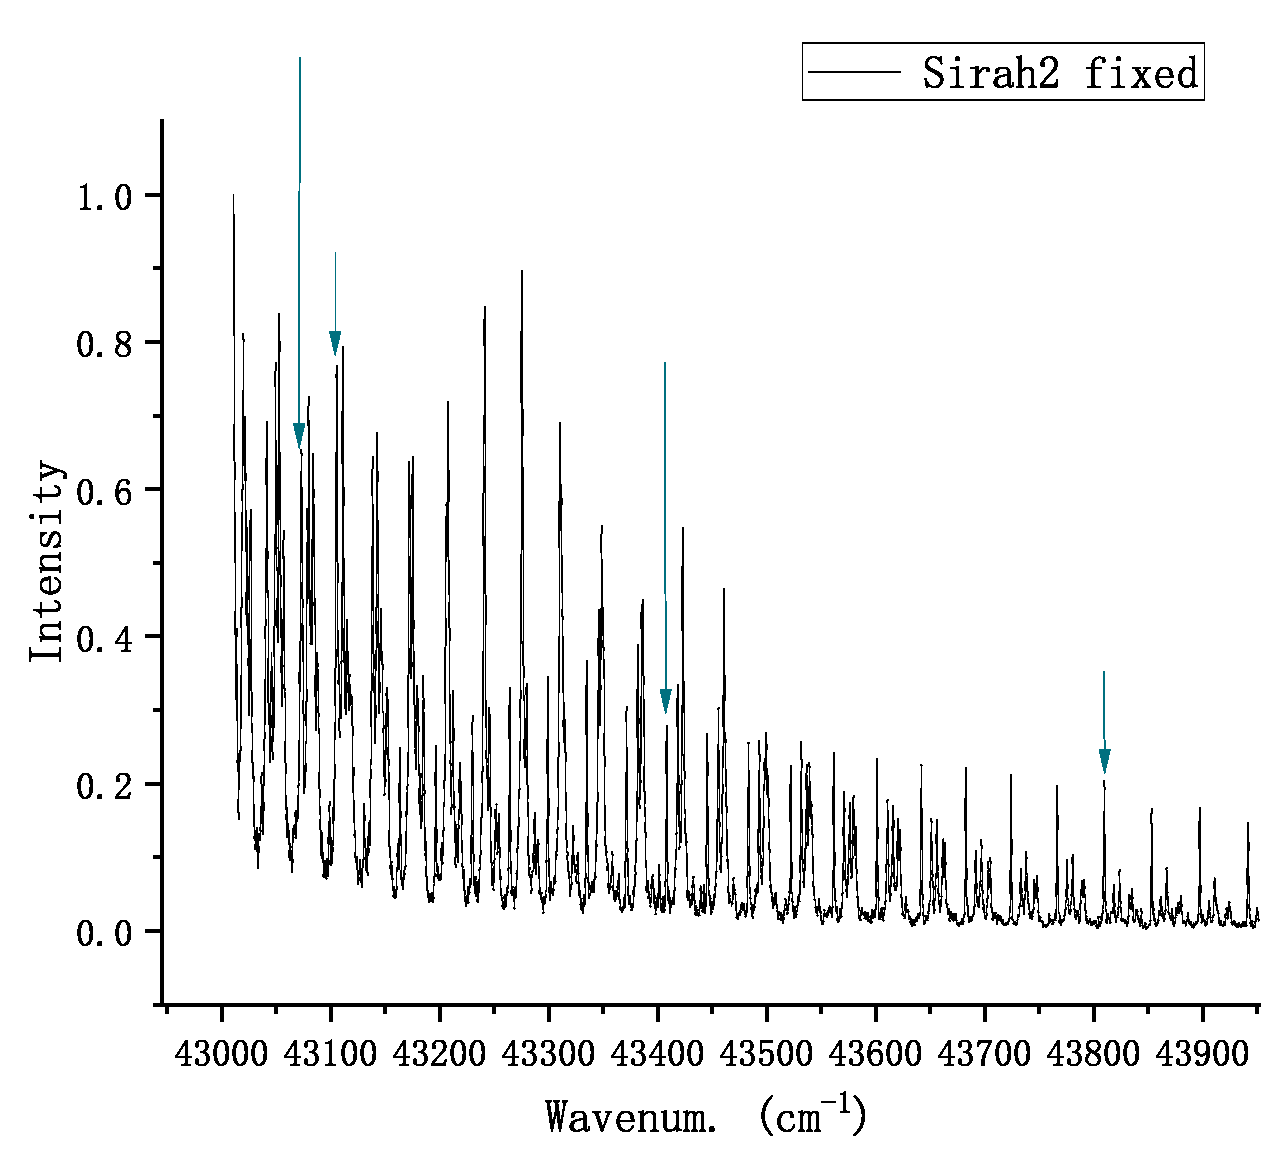
\includegraphics[width=0.6\textwidth]{scanmark.eps}};
			\filldraw[white] (-1.92,2.5) rectangle (-1.88,2.89);
			\node at (0.5,1.45){\textcolor[RGB]{0,112,127}{$\num{460.876}\unit{\nano \meter}$}};
			}
			\onslide<2>{\node at (-1.55,2){\includegraphics[width = 4cm]{gring460745.eps}};
			\node at (2.45,2){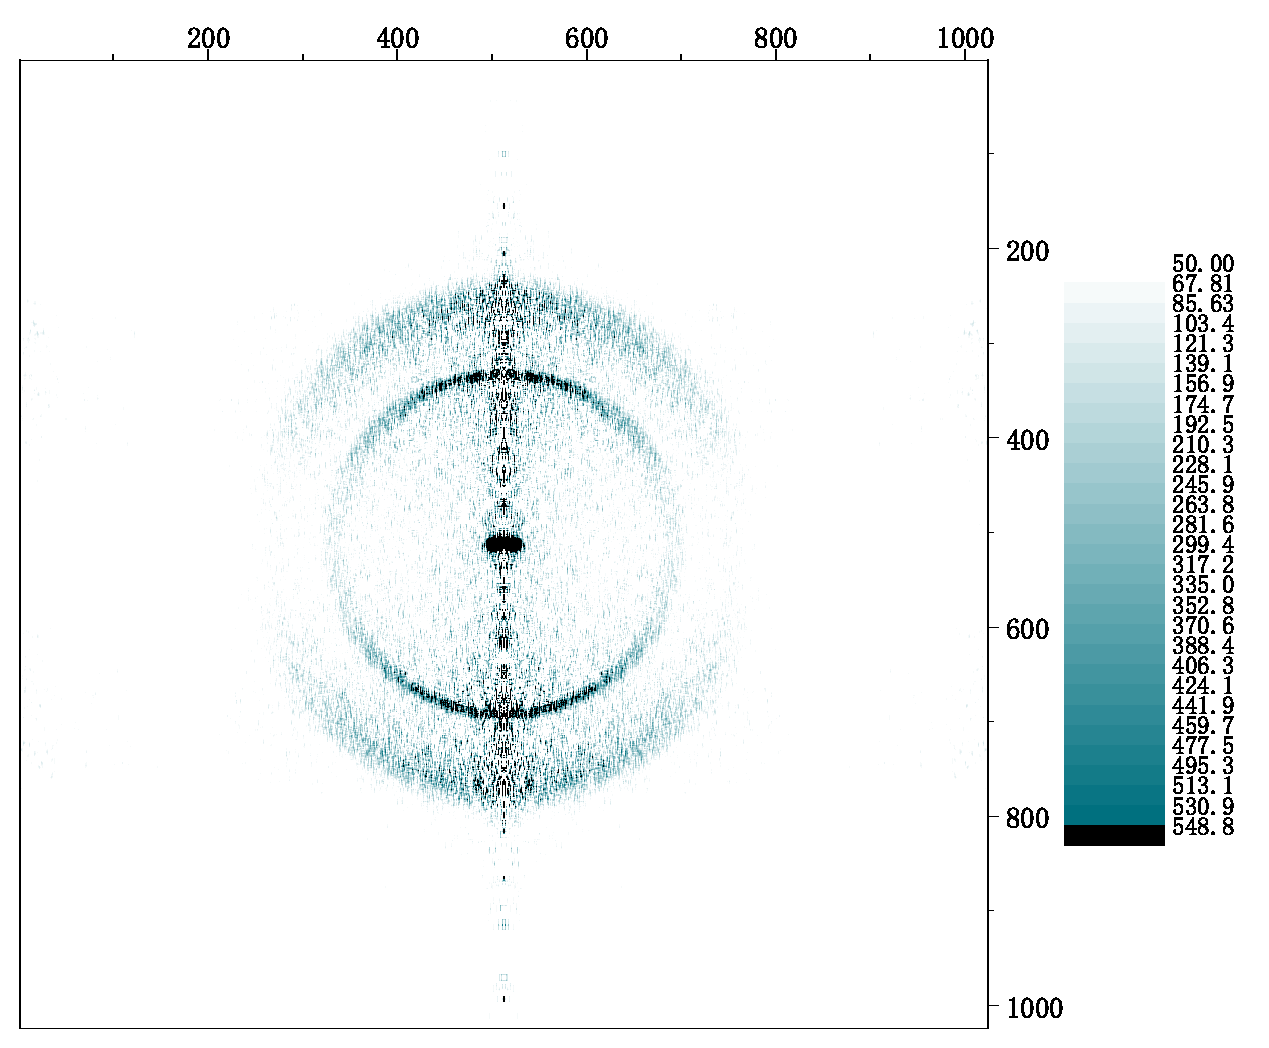
\includegraphics[width=4cm]{aring460745.eps}};
			\node at (-2,-2){\includegraphics[width=4cm]{rdis_peak_460745.eps}};
			\node at (2,-2){\includegraphics[width=4cm]{adis_460745b.eps}};
			\node at (1.3,-3.2){\textcolor[RGB]{0,112,127}{\small$\beta \approx 1.01$}};
				\node at (-3.0,3.3){\textcolor[RGB]{0,112,127}{smear}};
			\node at (3.07,3.3){\textcolor[RGB]{0,112,127}{Abel${}^{-1}$}};}
\end{tikzpicture}
\end{figure}
\end{frame}
\begin{frame}{Peak 4}
\begin{figure}[H]
\centering
\begin{tikzpicture}
		\onslide<1>{\node at (0,0){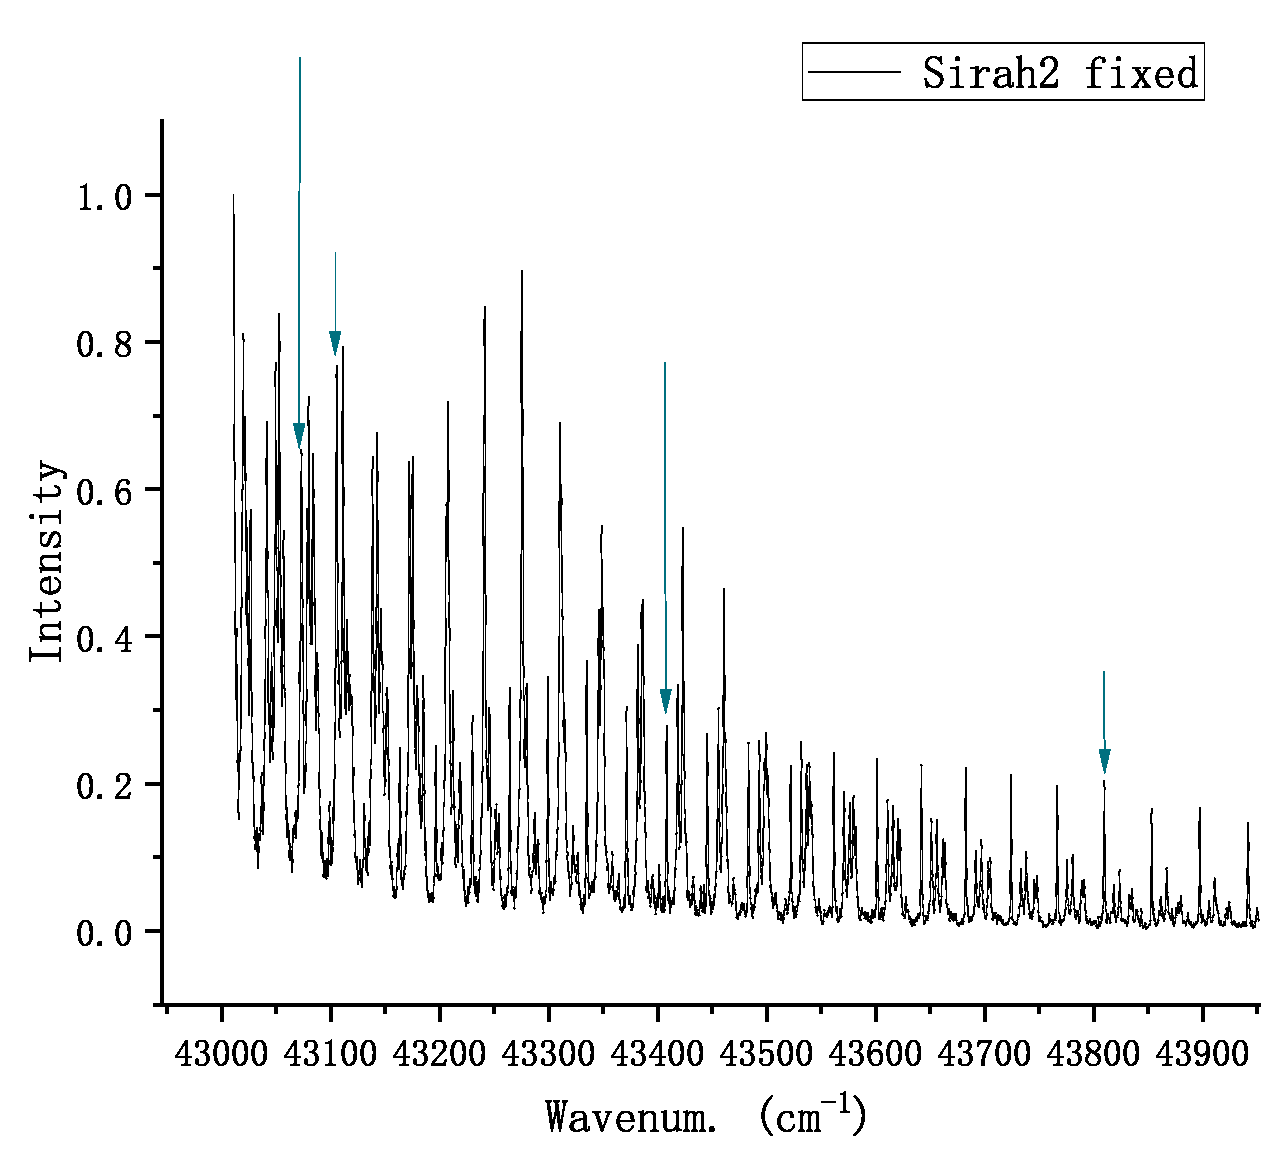
\includegraphics[width=0.6\textwidth]{scanmark.eps}};
			\filldraw[white] (-1.92,2.5) rectangle (-1.88,2.89);
			\node at (2.3,-0.25){\textcolor[RGB]{0,112,127}{$\num{456.653}\unit{\nano \meter}$}};
}
			\onslide<2>{\node at (-1.55,2){\includegraphics[width = 4cm]{gring456528.eps}};
			\node at (2.45,2){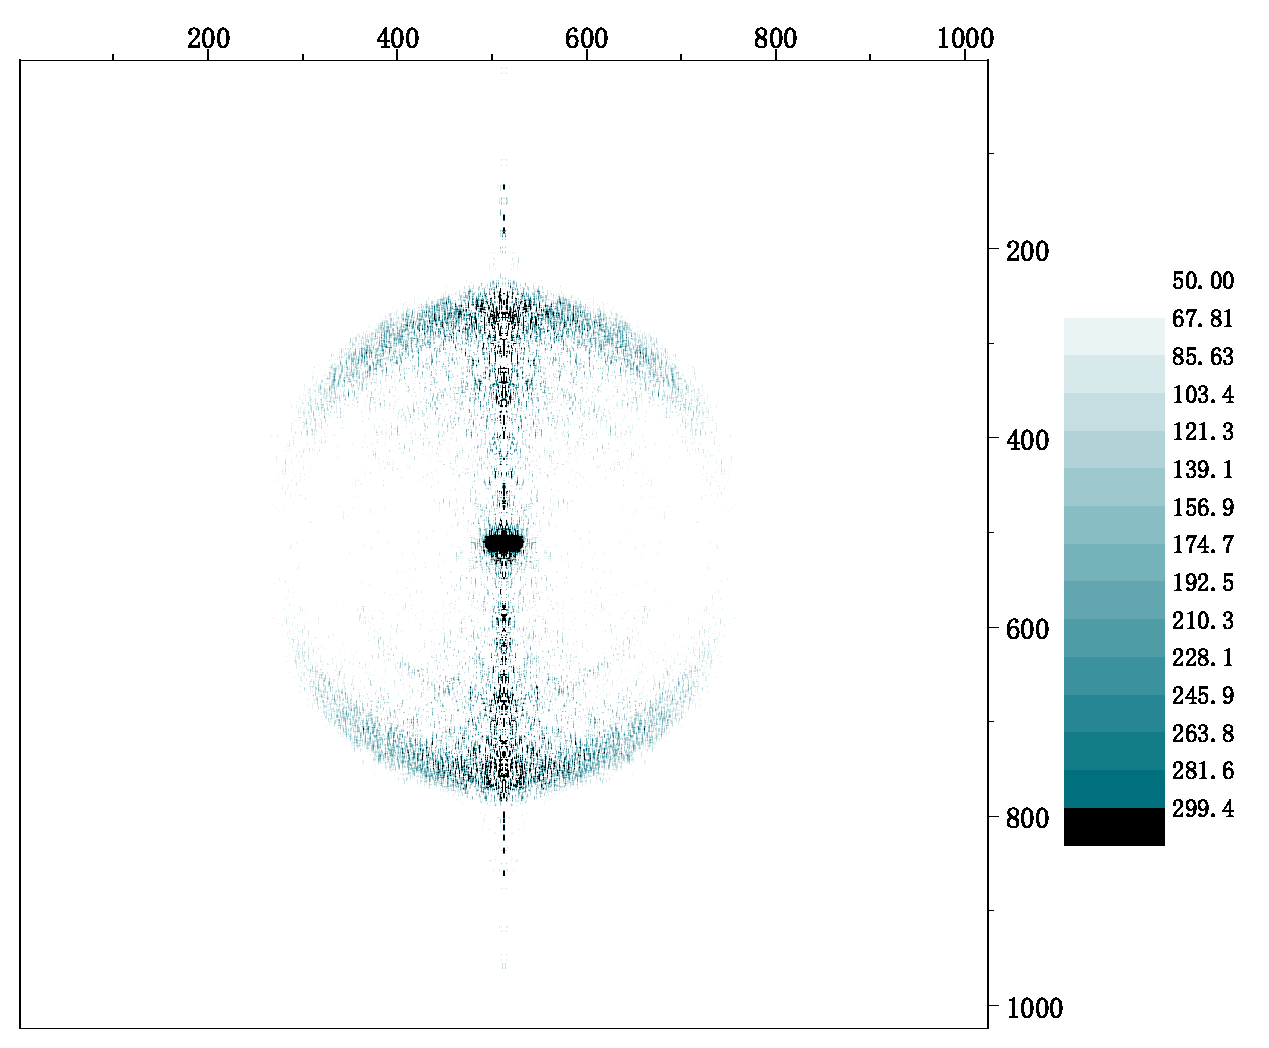
\includegraphics[width=4cm]{aring456528.eps}};
			\node at (-2,-2){\includegraphics[width=4cm]{rdis_peak_456528.eps}};
			\node at (2,-2){\includegraphics[width=4cm]{adis_456528b.eps}};
			\node at (1.3,-1.2){\small\textcolor[RGB]{0,112,127}{$\beta \approx 0.440$}};
				\node at (-3.0,3.3){\textcolor[RGB]{0,112,127}{smear}};
			\node at (3.07,3.3){\textcolor[RGB]{0,112,127}{Abel${}^{-1}$}};}
\end{tikzpicture}
\end{figure}
\end{frame}




%	
%	
%\begin{frame}
%	\begin{columns}
	%		\begin{column}{0.65\textwidth}
		%	
		%		\end{column}
	%		\vrule
	%		\begin{column}{0.35\textwidth}
		%			
		%		\end{column}
	%	\end{columns}
%\end{frame}
%	
%	
%	
%	
%
%	\begin{frame}
%		このスライドはソースコードが\qrcode[hyperlink,height=2cm]{https://github.com/xiaoyuleiba/Machinetime-Report}にて公開される。
%	\end{frame}
\end{document}









